\subsection*{STREAM}
\label{sec:stream}

STREAM~\cite{stream} is a centralised DSPS which tries to address the issue of long-running continuous queries. It
introduces a relational language called Continuous Query Language (CQL)~\cite{cql}, which allows the expression of
SQL-like queries over continuous data streams (Section~\ref{sec:cql}).  
Once a query is registered in the system, a correspondent \textit{query plan} is
compiled from it. Query plans are composed of \textit{operators}, which perform the actual processing, \textit{queues} which
buffer tuples as they move between operators, and \textit{synopses}, which store operator state. These elements are
composed to form a query plan implementing the CQL query. An example of query plan is depicted in Figure~\ref{fig:stream}. 
The incoming tuples are first stored in two sliding windows. Then they pass through two operators, first a \textsc{Join}
and then a \textsc{Select}. Synopsis are used by stateful operators to maintain some information about past tuples. In
between operators, tuples are always buffered using queues. Arrows represent data streams. 

\begin{figure}[b!]
	\centering
	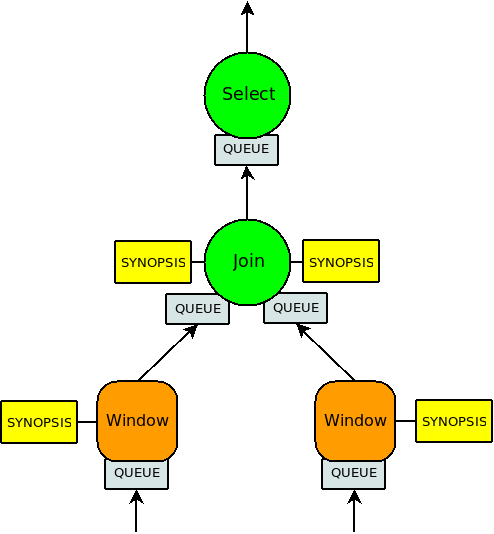
\includegraphics[width=0.5\textwidth]{img/stream.png} 
	\label{fig:stream}
	\caption{A simple query plan illustrating operators, queues, and synopses.} 
\end{figure} 

The major contribution of STREAM to the field is the introduction of CQL, that proved to be a very successful language. 
StreamSQL~\cite{streamsql}, an extension of CQL, is now considered the de-facto standard in stream processing.  

Being a centralised system, lacking the possibility to add resource to increase the processing capacity, STREAM made many
efforts to be as efficient as possible.  Within the engine massive stream and synopsis reuse is performed in order to
reduce the resource impact and maximise the number of queries executed on the node. Also some work has been done on the
scheduling of operators. While the first versions only included a round-robin policy, later a new algorithm called
\textit{chain scheduling}~\cite{stream-chains} has been introduced to minimize the memory footprint of the process. The
system also employs some approximations to deal with situation where the available resources are not sufficient to
support all the processing. In the event of overload, the system implements many approximation techniques to reduce the
quality of the results while continuing processing. STREAM also includes a graphical user interface which allow to
examine the query plan and to inspect the internal status of operators at run-time.

\paragraph{Considerations} 
STREAM has been a major contributor in the field of stream processing.
It introduced CQL, which allows the expression of complex queries with a simple declarative semantic, which become one
of the standards in the field of stream processing. I also plan to employ a declarative language in DISSP, an extension
of CQL, including the \emph{quality-metrics} described in Section~\ref{sec:metrics}.
STREAM also adopts several approximation techniques, to recover from CPU overload and memory shortage, like the ones described 
in Section~\ref{sec:dsps-approx}, which will be useful in the scope of my research.
